\chapter{Sistemas sensoriales}\label{ch:b3:sensory-systems}

En una noche oscura, el ojo humano detecta un destello de unos pocos
fotones ---la menor cantidad de luz que la física permite detectar. El
oído oye un sonido que desplaza el tímpano menos que el diámetro de un
átomo de hidrógeno, y distingue un tono de otro que difiere en una
quinta parte de un uno por ciento. Un perro sigue un rastro de unas
pocas moléculas por centímetro cúbico; un tiburón encuentra un lenguado
bajo la arena por el campo eléctrico de sus latidos. Todo sentido
empieza con una célula que convierte una clase de energía en un cambio
de potencial de membrana, y todo sentido termina como espigas en un
nervio; entre ambos extremos están los problemas que trata este
capítulo: cómo un receptor amplifica una sola molécula o un solo fotón
hasta una señal que una neurona pueda leer, cómo un intervalo de un
billón en intensidad se comprime en una frecuencia de unos cientos de
espigas por segundo, cómo una onda mecánica se clasifica por
frecuencia, cómo se distinguen diez mil olores con cuatrocientos
receptores y cómo el encéfalo, que nunca recibe otra cosa que espigas,
sabe de qué sentido proceden.

\section{Principios comunes a todos los sentidos}

\begin{definition}[Transducción, codificación y adaptación]\label{def:b3:sensory-systems:principles}
\index{transducción sensorial}\index{potencial receptor}\index{línea marcada}\index{campo receptivo}\index{adaptación!sensorial}\index{inhibición lateral}
Una \emph{célula receptora sensorial} contiene un mecanismo de
\emph{transducción} ---una proteína o una cascada--- que convierte un
estímulo (un fotón, una molécula, un desplazamiento, calor, un campo
eléctrico) en un cambio de conductancia de membrana y, por tanto, en un
\emph{potencial receptor}, graduado con el estímulo; la célula, o la
neurona sobre la que hace sinapsis, lo convierte en un tren de
potenciales de acción cuya frecuencia codifica la intensidad. La
\emph{modalidad} de una señal no la dan las espigas, idénticas en todos
los nervios, sino el cable por el que viajan y el lugar del encéfalo
donde ese cable termina: una \emph{línea marcada}. Una neurona
sensorial responde a estímulos situados dentro de un \emph{campo
receptivo} ---un trozo de piel, una región del campo visual, una banda
de frecuencias--- y los campos vecinos se afilan unos a otros mediante
la \emph{inhibición lateral}, en la que cada neurona suprime a sus
vecinas de modo que los bordes y los contrastes quedan exagerados. La
mayoría de los receptores se \emph{adaptan}: su respuesta a un estímulo
mantenido decae, de modo que informan del cambio y no del nivel, y su
intervalo de trabajo se desplaza para situarse en torno al fondo
dominante.
\end{definition}

\begin{theorem}[Weber, Fechner y Stevens]\label{thm:b3:sensory-systems:weber}
\index{ley de Weber}\index{ley de Fechner}\index{ley potencial de Stevens}
La observación de Weber (1834) es que el menor cambio detectable
$\Delta I$ en un estímulo de intensidad $I$ es una fracción fija de él:
$\Delta I/I = k$, con $k$ en torno a $0.02$ para el peso, $0.08$ para
el brillo y $0.1$ para la sonoridad. Si cada diferencia apenas
perceptible se cuenta como una unidad de sensación $S$, entonces $\mathrm{d}S = \mathrm{d}I/
(kI)$ y
\[
S = \frac{1}{k}\ln\frac{I}{I_{0}} ,
\]
donde $I_{0}$ es el umbral: la sensación crece como el logaritmo del
estímulo (Fechner, 1860), y por eso las intensidades se miden en
\omterm{def:b3:sensory-systems:cochlea}{decibelios} y en magnitudes, y por eso una vela añadida a otra vela se
nota y una vela añadida a un foco no. Los experimentos de escalado
directo, en los que los sujetos asignan números a las sensaciones, dan
en cambio una ley potencial $S \propto I^{n}$ (Stevens, 1957), con $n \approx
0.3$ para la sonoridad y el brillo, $1$ para la longitud de una línea y
$3.5$ para la descarga eléctrica; un logaritmo y una potencia pequeña
son casi indistinguibles a lo largo de unas pocas décadas, y ambas
leyes coinciden en lo esencial: el sistema nervioso comprime.
\end{theorem}
\begin{proof}
A partir de $\Delta I = kI$ para una unidad de $S$, el incremento de
sensación por incremento de estímulo es $\mathrm{d}S/\mathrm{d}I = 1/(kI)$;
integrando desde el umbral $I_{0}$, donde $S = 0$, resulta $S = (1/k)
\ln(I/I_{0})$. La ley potencial es la hipótesis alternativa de que una
\emph{razón} fija de estímulos produce una \emph{razón} fija de
sensaciones, $\mathrm{d}S/S = n\,\mathrm{d}I/I$, cuya integral es $S \propto I^{n}$;
para $n \to 0$ con un escalado adecuado tiende al logaritmo.
\end{proof}

\begin{omfigure}
\begin{tikzpicture}
\begin{axis}[
  width=0.68\linewidth, height=5.6cm,
  xmode=log,
  xmin=1, xmax=1e6, ymin=0, ymax=15,
  xlabel={intensidad del estímulo $I/I_{0}$}, ylabel={sensación $S$ (arbitraria)},
  xlabel style={font=\small, at={(axis description cs:0.5,-0.12)}, anchor=north}, ylabel style={font=\small},
  tick label style={font=\small}, ytick={0,5,10,15},
  clip=false,
]
\addplot[very thick, omDef, domain=1:1e6, samples=100] {ln(x)};
\addplot[very thick, omThm, domain=1:1e6, samples=100] {0.235*x^0.3 - 0.235};
\addplot[very thick, omMeth!70!black, domain=1:1e6, samples=100] {0.5*x^0.24 - 0.5};
\node[font=\scriptsize, omDef, anchor=north west] at (axis cs:2,10.2) {Fechner: $S = \ln(I/I_{0})$};
\node[font=\scriptsize, omThm, anchor=south east] at (axis cs:9e5,0.4) {Stevens: $S \propto I^{0.3}$};
\node[font=\scriptsize, omMeth!70!black, anchor=north west] at (axis cs:2,12.5) {Stevens: $S \propto I^{0.24}$};
\end{axis}
\end{tikzpicture}

{\small Compresión de un intervalo de intensidad de un millón en una
sensación que crece despacio: el logaritmo de Fechner y las \omterm{thm:b3:sensory-systems:weber}{leyes
potenciales de Stevens} con exponentes pequeños son difíciles de
distinguir a lo largo de unas pocas décadas, y ambas dicen que los
sentidos informan de razones, no de diferencias.}
\end{omfigure}

\section{La visión}

\begin{definition}[La retina]\label{def:b3:sensory-systems:retina}
\index{retina}\index{bastón}\index{cono}\index{fototransducción}\index{rodopsina}\index{célula ganglionar}\index{centro--periferia}
La \emph{retina} es una lámina de encéfalo en el fondo del ojo, tres
capas de células con los fotorreceptores, paradójicamente, al fondo,
contra el epitelio pigmentario. Los \emph{bastones} ---$10^{8}$ por
ojo, un solo pigmento, la \emph{rodopsina}--- sirven a la luz tenue y
se saturan a la luz del día; los \emph{conos} ---$6\times 10^{6}$, tres
pigmentos con máximos en el azul, el verde y el rojo, apretados en la
fóvea--- sirven a la luz del día, al color y a la agudeza. La
\emph{fototransducción} es una cascada: un fotón isomeriza el cromóforo
retinal de una rodopsina; la rodopsina activada enciende centenares de
moléculas de la proteína~G transducina, cada una de las cuales activa
una fosfodiesterasa que destruye el GMP cíclico; la caída del GMPc
cierra los canales catiónicos que el GMPc mantenía abiertos en la
oscuridad, la ``corriente de oscuridad'' entrante se detiene y la
célula se \emph{hiperpolariza}: la luz apaga un fotorreceptor, que
libera menos glutamato. En la oscuridad la célula está despolarizada y
liberando sin cesar. La señal pasa a las \emph{células bipolares} (de
tipo ON y OFF, que la invierten o la conservan) y de ahí a las
\emph{células ganglionares}, un millón por ojo, cuyos axones forman el
nervio óptico ---una compresión de cien veces. Las células
horizontales y amacrinas conectan lateralmente, y su inhibición da a
cada célula ganglionar un \omterm{def:b3:sensory-systems:principles}{campo receptivo} de \emph{centro--periferia}:
excitado por la luz en un disco central e inhibido por la luz en el
anillo que lo rodea (o al revés), de modo que la retina informa del
contraste local y de los bordes, y no de la luz absoluta.
\end{definition}

\begin{omfigure}
\begin{tikzpicture}[every node/.style={font=\scriptsize}, >=stealth]
  % cascade boxes with amplification numbers
  \node[draw, thick, rounded corners, fill=omProp!30, align=center] (ph) at (0,0) {1 fotón};
  \node[draw, thick, rounded corners, fill=omDef!20, align=center] (rh) at (2.6,0) {1 rodopsina*\\(metarrodopsina II)};
  \node[draw, thick, rounded corners, fill=omDef!20, align=center] (tr) at (5.6,0) {$\sim 500$ transducinas\\activadas};
  \node[draw, thick, rounded corners, fill=omDef!20, align=center] (pde) at (8.6,0) {$\sim 500$ PDE activas:\\$\sim 10^{5}$ GMPc hidrolizados};
  \node[draw, thick, rounded corners, fill=omThm!20, align=center] (ch) at (5.6,-2.0) {se cierran $\sim 200$ canales catiónicos;\\la corriente de oscuridad cae \qty{1}{pA}};
  \node[draw, thick, rounded corners, fill=omMeth!25, align=center] (out) at (1.4,-2.0) {hiperpolarización de \qty{1}{mV};\\se libera menos glutamato};
  \draw[->, thick] (ph) -- (rh); \draw[->, thick] (rh) -- (tr); \draw[->, thick] (tr) -- (pde);
  \draw[->, thick] (pde.south) |- (ch.east); \draw[->, thick] (ch) -- (out);
  \node[below, font=\tiny, align=center] at (7.1,-2.8) {cada paso multiplica; toda la cascada se apaga en \qty{200}{ms} por obra de la\\rodopsina cinasa, la arrestina y la GTPasa de la transducina, y luego se reinicia};
\end{tikzpicture}

{\small La \omterm{def:b3:sensory-systems:retina}{fototransducción} como amplificador. Un solo fotón absorbido
cierra centenares de canales a través de dos etapas catalíticas, una
ganancia de alrededor de un millón en moléculas ---suficiente para que
un único fotón produzca una corriente medible en un \omterm{def:b3:sensory-systems:retina}{bastón}.}
\end{omfigure}

\begin{theorem}[Contar fotones: la frecuencia de visión]\label{thm:b3:sensory-systems:hecht}
\index{detección de un solo fotón}\index{curva de frecuencia de visión}\index{Poisson!recuento de fotones}
Un destello que entrega en promedio $a$ fotones absorbidos a un grupo
de bastones entrega, en cualquier presentación concreta, un número $k$
que sigue una distribución de Poisson: $P(k) = e^{-a}a^{k}/k!$. Si el
observador declara ver el destello siempre que se absorben al menos $n$
fotones, la probabilidad de ver es
\[
P_{\text{ver}}(a) = 1 - \sum_{k=0}^{n-1} e^{-a}\,\frac{a^{k}}{k!} ,
\]
una curva que sube de $0$ a $1$ a medida que $a$ crece y cuya
\emph{pendiente} en una escala logarítmica de $a$ depende solo de $n$:
cuanto mayor es el recuento umbral, más empinada es la curva. Ajustar
la curva medida de frecuencia de visión da, por tanto, $n$ sin saber
cuántos de los fotones entregados fueron absorbidos realmente.
\end{theorem}
\begin{proof}
Los fotones de una fuente débil y constante llegan de forma
independiente y al azar, y el número absorbido en un destello breve a
partir de una media de $a$ es de Poisson (el límite de una binomial con
muchos fotones, cada uno absorbido con probabilidad pequeña). Ver exige
$k \ge n$, cuya probabilidad es uno menos la suma de los $n$ primeros
términos de Poisson. Escalar la fuente por un factor $c$ multiplica $a$
por $c$ y desplaza la curva a lo largo del eje $\log a$ sin cambiar su
forma, de modo que la forma identifica $n$: para $n =
1$, $P = 1 - e^{-a}$ sube a lo largo de dos décadas de $a$; para $n = 6$
sube a lo largo de menos de una.
\end{proof}

\begin{proof}[Evidencia]
Hecht, Shlaer y Pirenne (1942) sentaron a los observadores en la
oscuridad durante media hora y luego proyectaron durante un
milisegundo un diminuto punto verde sobre la periferia de la \omterm{def:b3:sensory-systems:retina}{retina},
rica en bastones, cientos de veces y a varias intensidades, y
registraron la fracción de destellos vistos. El destello umbral
contenía, en la córnea, unos $90$ fotones, de los cuales (tras la
reflexión, la absorción en los medios del ojo y la probabilidad del
$20\,\%$ de que un fotón que llega a un \omterm{def:b3:sensory-systems:retina}{bastón} sea absorbido por la
\omterm{def:b3:sensory-systems:retina}{rodopsina}) se absorbían unos $5$--$14$. Las \omterm{thm:b3:sensory-systems:hecht}{curvas de frecuencia de
visión} tenían la pendiente de $n = 5$ a $7$: el observador decía
``sí'' cuando unos seis bastones, de los quinientos situados bajo el
punto, habían capturado cada uno un solo fotón. Un \omterm{def:b3:sensory-systems:retina}{bastón} detecta un
fotón; el encéfalo exige unos pocos en coincidencia, para mantener las
falsas alarmas procedentes de las isomerizaciones espontáneas de los
bastones ---una por \omterm{def:b3:sensory-systems:retina}{bastón} cada cuarenta segundos--- por debajo del
ritmo de las estrellas.
\end{proof}

\begin{omfigure}
\begin{tikzpicture}
\begin{axis}[
  width=0.68\linewidth, height=5.6cm,
  xmode=log,
  xmin=0.1, xmax=100, ymin=0, ymax=1.05,
  xlabel={fotones absorbidos por destello, en media, $a$}, ylabel={probabilidad de ver},
  xlabel style={font=\small, at={(axis description cs:0.5,-0.12)}, anchor=north}, ylabel style={font=\small},
  tick label style={font=\small}, ytick={0,0.5,1},
  clip=false,
]
\addplot[very thick, omDef, domain=0.1:100, samples=120] {1-exp(-x)};
\addplot[very thick, omProp, domain=0.1:100, samples=120] {1-exp(-x)*(1+x+x^2/2)};
\addplot[very thick, omThm, domain=0.1:100, samples=120] {1-exp(-x)*(1+x+x^2/2+x^3/6+x^4/24+x^5/120)};
\node[font=\scriptsize, omDef, anchor=north west] at (axis cs:0.12,0.95) {$n = 1$};
\node[font=\scriptsize, omProp, anchor=north west] at (axis cs:1.1,0.5) {$n = 3$};
\node[font=\scriptsize, omThm, anchor=north west] at (axis cs:5.5,0.45) {$n = 6$};
\end{axis}
\end{tikzpicture}

{\small \omterm{thm:b3:sensory-systems:hecht}{Curvas de frecuencia de visión} para umbrales de uno, tres y
seis fotones absorbidos. Cuanto más empinada es la curva, más fotones
deben coincidir; los observadores de Hecht dieron curvas como la roja.}
\end{omfigure}

\begin{omfigure}
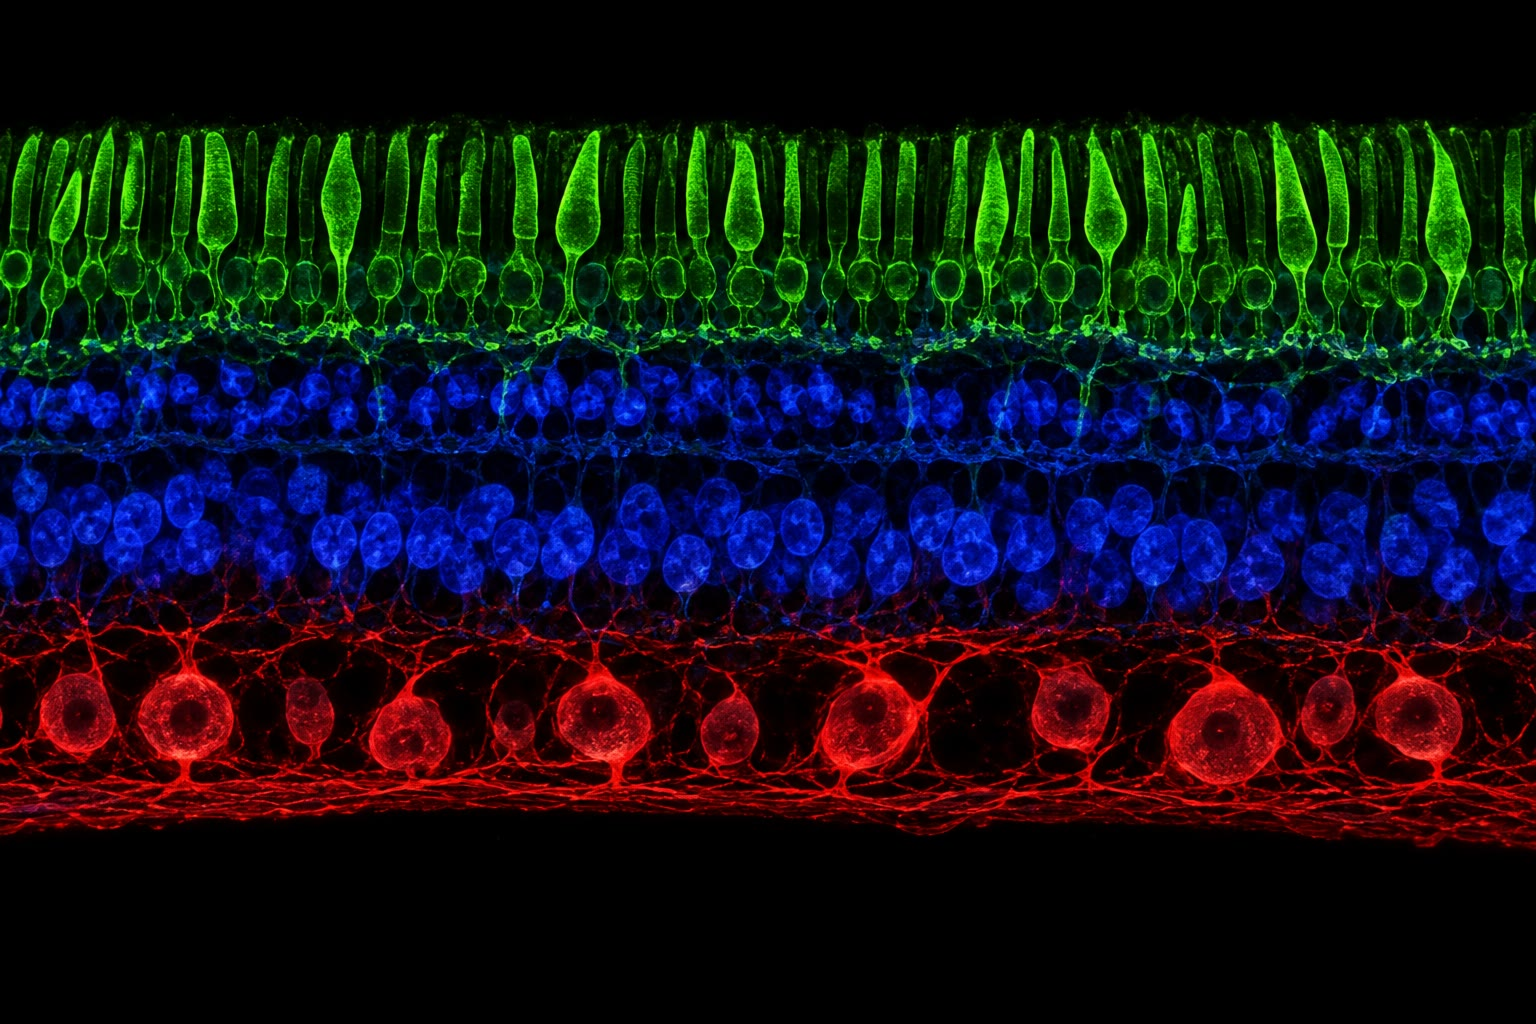
\includegraphics[width=0.46\linewidth]{images/book5/ai/b5-18-retina-section.jpg}\hspace{0.04\linewidth}
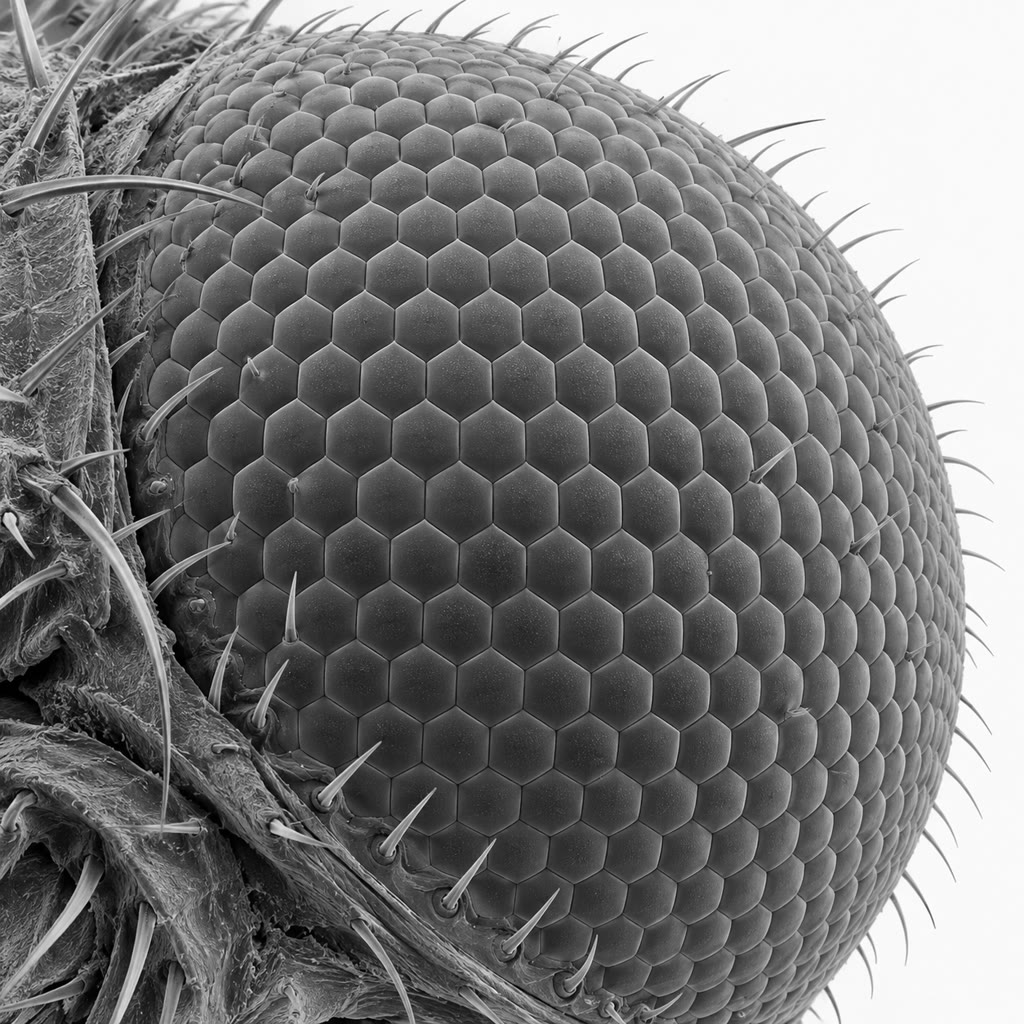
\includegraphics[width=0.36\linewidth]{images/book5/ai/b5-18-compound-eye.jpg}

{\small Izquierda: un corte de la \omterm{def:b3:sensory-systems:retina}{retina}, con los fotorreceptores
(verde) al fondo, luego las células bipolares y horizontales, y luego
las \omterm{def:b3:sensory-systems:retina}{células ganglionares} (rojo), cuyos axones parten hacia el encéfalo.
Derecha: el ojo compuesto de una mosca, con centenares de lentes
separadas, cada una con sus propios receptores ---una solución distinta
al mismo problema.}
\end{omfigure}

\section{La audición y el equilibrio}

\begin{definition}[La cóclea]\label{def:b3:sensory-systems:cochlea}
\index{cóclea}\index{membrana basilar}\index{tonotopía}\index{célula ciliada}\index{estereocilios}\index{enlace apical}\index{decibelio}
El sonido es una onda de presión; el problema del oído es detectar
cambios de presión de unas pocas decenas de micropascales en el aire y
clasificarlos por frecuencia. El tímpano y los tres huesecillos del
oído medio concentran la fuerza desde los \qty{55}{mm^2} del tímpano
sobre los \qty{3}{mm^2} de la ventana oval, y elevan la presión unas
veinte veces ---la adaptación de impedancias entre el aire y el líquido
del oído interno, sin la cual la mayor parte del sonido se reflejaría.
Dentro de la \emph{cóclea}, un tubo enrollado de \qty{35}{mm} de
longitud, la onda de presión viaja a lo largo de la \emph{membrana
basilar}, que es estrecha y rígida en la base y ancha y flexible en el
ápice; cada frecuencia hace vibrar la membrana sobre todo en un lugar
---las frecuencias altas cerca de la base, las bajas cerca del ápice---,
un mapa \emph{tonotópico} que el encéfalo lee como tono. Sobre la
membrana se asientan las \emph{células ciliadas}: \num{3500} células
ciliadas internas en una sola fila, cada una coronada por un haz de
\emph{estereocilios} unidos punta con punta por finos \emph{enlaces
apicales}; doblar el haz hacia su \omterm{def:b3:cytoskeleton-motility:cilia}{cilio} más alto estira los enlaces y
abre canales catiónicos en microsegundos, sin segundo mensajero alguno,
y el potasio entra desde la endolinfa, cuya composición insólita y cuyo
potencial de $+\qty{80}{mV}$ dan una fuerza impulsora de \qty{150}{mV}.
Las células ciliadas internas envían la señal al nervio auditivo; las
\num{12000} células ciliadas externas, movidas por el mismo
desplazamiento, se contraen y se alargan con el sonido gracias a la
proteína motora prestina y devuelven energía a la vibración de la
membrana ---un amplificador que afila el ajuste cien veces y que es lo
que falla en la mayoría de las sorderas. La intensidad se mide en
\emph{decibelios}: $L = 10\log_{10}
(I/I_{0})$, con $I_{0} = \qty{1e-12}{W/m^2}$ el umbral de audición; el
oído funciona a lo largo de \qty{120}{dB}, un billón en intensidad.
\end{definition}

\begin{omfigure}
\begin{tikzpicture}[every node/.style={font=\scriptsize}, >=stealth]
  % unrolled cochlea
  \begin{scope}
    \draw[thick, omDef, fill=omDef!10] (0,0.9) -- (7,1.4) -- (7,-1.4) -- (0,-0.9) -- cycle;
    \draw[very thick, omProp] (0,0.15) -- (7,-0.15); \draw[very thick, omProp] (0,-0.15) -- (7,0.15);
    \node[above] at (0.8,1.05) {base: estrecha, rígida}; \node[above] at (6.2,1.5) {ápice: ancha, flexible};
    \node[left, align=right] at (-0.1,0) {ventana oval\\(desde el estribo)};
    \foreach \x/\f in {0.9/\qty{16}{kHz}, 2.3/\qty{4}{kHz}, 3.8/\qty{1}{kHz}, 5.4/\qty{250}{Hz}, 6.6/\qty{60}{Hz}} { \draw[omThm, thick] (\x,-0.55) -- (\x,0.55); \node[below, omThm] at (\x,-0.65) {\f}; }
    \node[below, align=center] at (3.5,-1.7) {membrana basilar (naranja): cada frecuencia\\vibra sobre todo en un lugar --- tonotopía};
  \end{scope}
  % hair cell mechanism
  \begin{scope}[xshift=8.2cm, yshift=-0.6cm]
    \draw[thick, fill=omMeth!20] (0,0) rectangle (1.6,1.2); \node[below] at (0.8,-0.05) {célula ciliada};
    \foreach \x/\h in {0.35/0.6, 0.65/0.85, 0.95/1.1, 1.25/1.35} \draw[very thick, omMeth!70!black] (\x,1.2) -- (\x,1.2+\h);
    \foreach \x/\h/\xx/\hh in {0.35/0.6/0.65/0.85, 0.65/0.85/0.95/1.1, 0.95/1.1/1.25/1.35} \draw[omThm, thick] (\x,1.2+\h) -- (\xx,1.2+\hh-0.1);
    \draw[->, thick] (1.9,2.3) -- (2.4,2.3) node[right, align=left, font=\tiny] {doblar hacia el más alto:\\los enlaces se estiran,\\los canales se abren\\en $\unit{\micro s}$; entra K$^{+}$\\(impulso de \qty{150}{mV})};
    \node[above, align=center] at (0.8,2.7) {estereocilios unidos\\por enlaces apicales (rojo)};
  \end{scope}
\end{tikzpicture}

{\small Izquierda: la \omterm{def:b3:sensory-systems:cochlea}{cóclea} desenrollada ---la \omterm{def:b3:sensory-systems:cochlea}{membrana basilar} pasa
de rígida a flexible, y cada frecuencia alcanza su máximo en su propio
lugar. Derecha: un haz ciliar, cuyos \omterm{def:b3:sensory-systems:cochlea}{enlaces apicales} abren
mecánicamente los canales de transducción cuando el haz se dobla.}
\end{omfigure}

\begin{proof}[Evidencia]
Von Békésy (en la década de 1940) abrió las \omterm{def:b3:sensory-systems:cochlea}{cócleas} de cadáveres,
espolvoreó partículas de plata sobre la \omterm{def:b3:sensory-systems:cochlea}{membrana basilar} y observó bajo
luz estroboscópica cómo los tonos puros levantaban una onda viajera
cuyo máximo quedaba tanto más cerca de la base cuanto más agudo era el
tono ---el código de lugar, por el que recibió el premio Nobel en 1961.
Hudspeth (en la década de 1980) empujó un solo haz ciliar con una fibra
de vidrio y registró la corriente: fluía antes de \qty{10}{\micro s}
desde el empujón, demasiado rápido para cualquier cascada enzimática,
en proporción a cuánto se desplazaba el haz hacia su fila más alta, y
desaparecía cuando los \omterm{def:b3:sensory-systems:cochlea}{enlaces apicales} se cortaban con un quelante de
calcio. La apertura es mecánica ---el enlace tira del canal y lo
abre---, y por eso la audición es el más rápido de los sentidos y por
eso su transductor lo destruyen los sonidos fuertes que rompen los
enlaces.
\end{proof}

\begin{example}[Los números del oído]\label{ex:b3:sensory-systems:ear-numbers}
En el umbral de audición la \omterm{def:b3:sensory-systems:cochlea}{membrana basilar} se desplaza unos
\qty{0.1}{nm} y la amplitud de presión es de \qty{20}{\micro Pa}, una
dosmilmillonésima de la atmosférica; a \qty{120}{dB} la presión es un
millón de veces mayor y el movimiento de la membrana, de decenas de
nanómetros. Un oído joven oye desde \qty{20}{Hz} hasta \qty{20}{kHz} y
separa tonos que distan un \qty{0.3}{\%}, con la discriminación del
código de lugar afilada por las \omterm{def:b3:sensory-systems:cochlea}{células ciliadas} externas. Las
\num{30000} fibras del nervio auditivo descargan al compás de la onda
de presión hasta unos \qty{4}{kHz} (enganche de fase) y transportan una
información temporal con precisión de decenas de microsegundos, a
partir de la cual el encéfalo calcula la dirección de un sonido por la
diferencia de llegada a los dos oídos ---de tan solo \qty{10}{\micro s}.
Los órganos del equilibrio emplean las mismas \omterm{def:b3:sensory-systems:cochlea}{células ciliadas}: en los
\emph{canales semicirculares} la inercia del líquido las dobla cuando
la cabeza gira (aceleración angular), y en los órganos otolíticos una
capa de cristales de carbonato de calcio las carga con la gravedad y la
aceleración lineal.
\end{example}

\begin{omfigure}
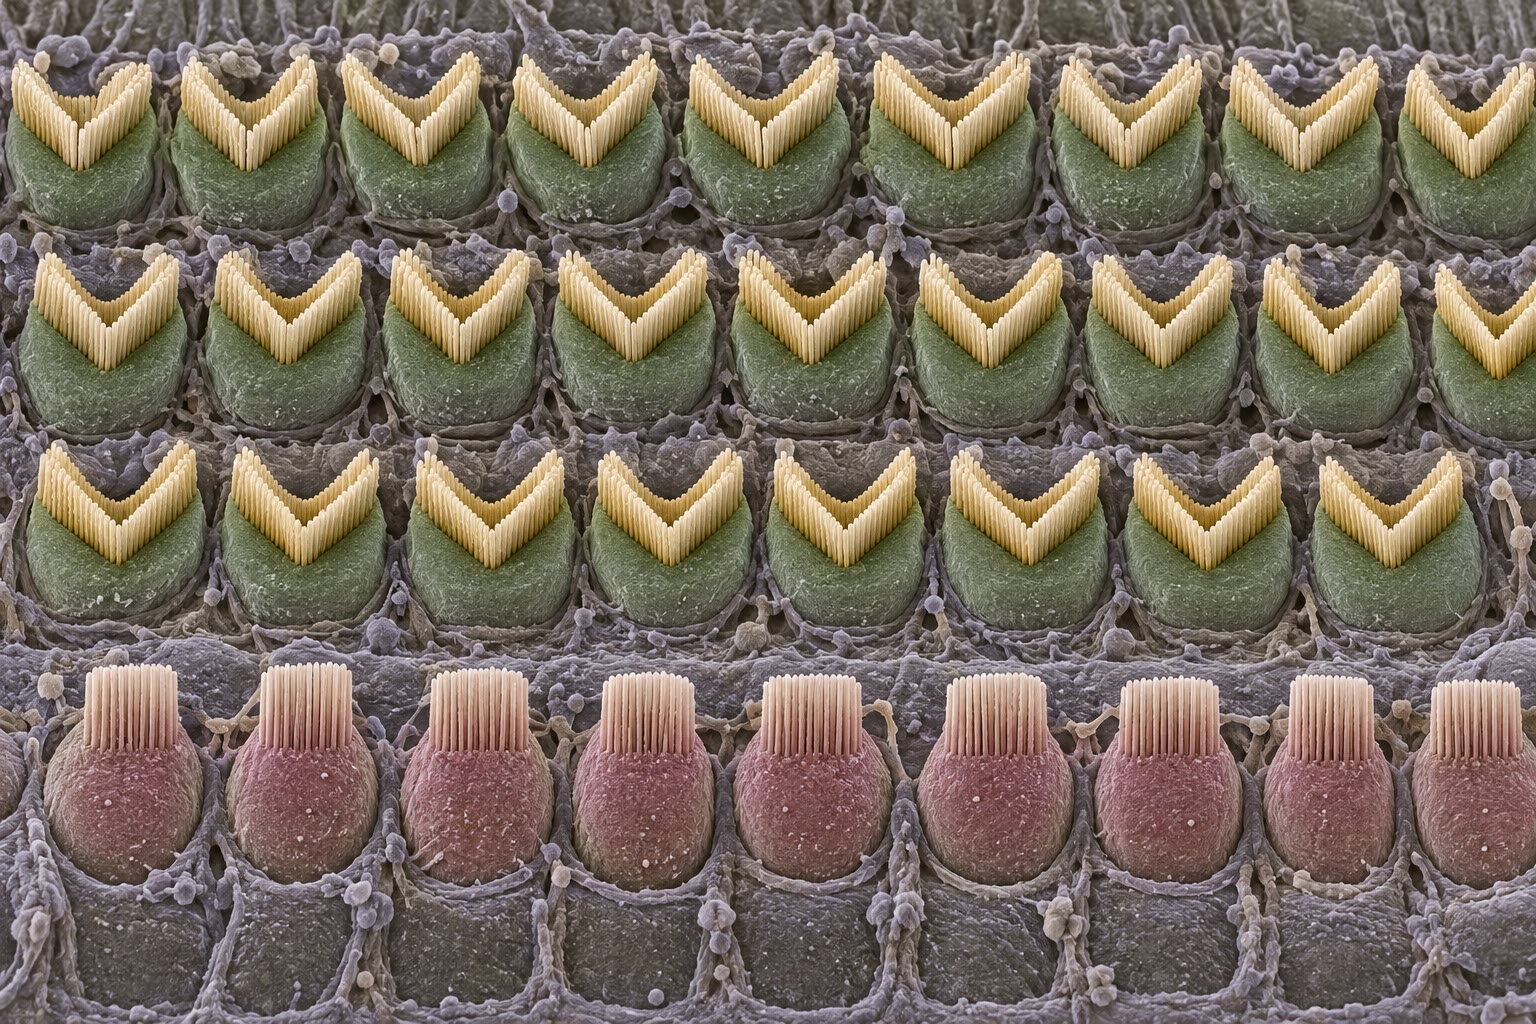
\includegraphics[width=0.54\linewidth]{images/book5/ai/b5-18-cochlea-hair-cells.jpg}

{\small El órgano de Corti visto desde arriba: tres filas de \omterm{def:b3:sensory-systems:cochlea}{células
ciliadas} externas con haces en forma de V, y una fila de \omterm{def:b3:sensory-systems:cochlea}{células
ciliadas} internas. Los \omterm{def:b3:sensory-systems:cochlea}{enlaces apicales} de cada haz abren los canales;
las células externas amplifican, las internas informan.}
\end{omfigure}

\section{Los sentidos químicos}

\begin{definition}[El olfato y el gusto]\label{def:b3:sensory-systems:chemical}
\index{receptor olfativo}\index{código combinatorio}\index{glomérulo}\index{gusto}
El olfato empieza en un trozo de epitelio situado en lo alto de la
nariz, donde unos diez millones de \emph{neuronas sensoriales
olfativas} expresan cada una un gen de \emph{receptor olfativo} de los
aproximadamente $400$ del ser humano (\num{1100} en el ratón, la mayor
familia génica de uno y otro genoma) ---receptores acoplados a
proteínas~G que fijan moléculas odorantes en un bolsillo y, a través
del AMP cíclico, abren un canal. Cada receptor fija varios odorantes y
cada odorante se fija a varios receptores, de modo que un olor es un
\emph{código combinatorio}, un patrón de actividad repartido entre los
$400$ tipos de receptor, y cambiar un carbono en una molécula cambia el
patrón y el olor. Todas las neuronas que expresan un receptor envían
sus axones al mismo \emph{glomérulo}, o a los dos mismos, del bulbo
olfativo, de manera que el bulbo alberga un mapa en el que cada olor es
un patrón espacial de glomérulos activos, leído por la corteza sin
pasar por el \omterm{def:b3:nervous-systems:plan}{tálamo}. El gusto es más simple: cinco modalidades, cada
una una \omterm{def:b3:sensory-systems:principles}{línea marcada} desde sus propias células receptoras ---el dulce,
el umami y el amargo a través de receptores acoplados a proteínas~G
(un receptor del dulce, uno del umami y unos veinticinco del amargo),
el salado a través de un canal de sodio y el ácido a través de un canal
de protones---, y el resto de lo que llamamos sabor es olfato, que
alcanza la nariz por el fondo de la boca.
\end{definition}

\begin{proof}[Evidencia]
Buck y Axel (1991) razonaron que los receptores de odorantes serían
receptores acoplados a proteínas~G expresados solo en el epitelio
olfativo, y hallaron mediante PCR con \omterm{def:b3:genetic-engineering:pcr}{cebadores} degenerados una familia
de centenares de esos genes, expresados allí y en ningún otro sitio
---los receptores del olfato, desconocidos durante un siglo. La
hibridación in situ mostró un receptor por neurona y la convergencia de
las neuronas semejantes en \omterm{def:b3:sensory-systems:chemical}{glomérulos} únicos; Malnic, Buck y sus
colaboradores (1999) registraron neuronas aisladas y mostraron que cada
odorante activaba varios tipos de receptor y cada receptor, varios
odorantes ---el \omterm{def:b3:sensory-systems:chemical}{código combinatorio}. Bushdid y sus colaboradores (2014)
pidieron a los sujetos que discriminaran mezclas y estimaron que el ser
humano puede distinguir más de un billón de olores, muy por encima de
los pocos miles de la creencia común.
\end{proof}

\begin{proposition}[La capacidad de un código combinatorio]\label{prop:b3:sensory-systems:combinatorial}
\index{código combinatorio!capacidad}
Con $R$ tipos de receptor, cada uno activo o en silencio, un olor puede
representarse mediante cualquiera de $2^{R}$ patrones; con $R = 400$
eso da $10^{120}$, e incluso si solo se consideran los patrones con
exactamente $10$ tipos activos hay
$\binom{400}{10} \approx 3\times 10^{20}$. La discriminación no la
limita el código, sino el ruido de los receptores y la lectura que hace
el encéfalo: un código de \omterm{def:b3:sensory-systems:principles}{líneas marcadas} con un receptor por olor
permitiría $400$ olores; uno combinatorio permite más de los que hay
moléculas que oler. El precio es que un receptor aislado dice poco al
encéfalo por su cuenta; el patrón ha de leerse como un todo, que es lo
que hacen el mapa glomerular y la corteza olfativa.
\end{proposition}

\begin{omfigure}
\begin{tikzpicture}[every node/.style={font=\scriptsize}, >=stealth]
  % receptor rows, odorant columns
  \foreach \i/\lab in {1/receptor~A, 2/receptor~B, 3/receptor~C, 4/receptor~D, 5/receptor~E} \node[left] at (-0.1,-0.7*\i) {\lab};
  \foreach \j/\lab in {1/hexanol, 2/heptanol, 3/octanol, 4/limoneno} \node[above, rotate=0] at (1.2*\j-0.6,-0.35) {\lab};
  \foreach \i/\j/\v in {1/1/100, 1/2/30, 2/1/60, 2/2/100, 2/3/50, 3/2/40, 3/3/100, 3/4/20, 4/3/70, 5/4/100, 1/4/30} \fill[omThm!\v] (1.2*\j-1.15,-0.7*\i-0.3) rectangle (1.2*\j-0.05,-0.7*\i+0.3);
  \foreach \i in {1,...,5} \foreach \j in {1,...,4} \draw[gray!50] (1.2*\j-1.15,-0.7*\i-0.3) rectangle (1.2*\j-0.05,-0.7*\i+0.3);
  \node[below, align=center] at (2.1,-4.1) {cada odorante activa un conjunto de receptores,\\cada receptor un conjunto de odorantes:\\el olor es la columna};
  % glomerular map
  \begin{scope}[xshift=9.2cm, yshift=-2.2cm]
    \draw[thick, omDef!60, fill=omDef!8] (0,0) ellipse (2.6 and 1.7); \node[above] at (0,1.75) {bulbo olfativo: glomérulos};
    \foreach \p in {(-1.8,0.6),(-1.0,1.0),(-0.2,0.7),(0.8,1.0),(1.7,0.5),(-1.6,-0.4),(-0.6,-0.6),(0.4,-0.3),(1.3,-0.7),(0.1,0.2)} \draw[omDef!70, fill=omDef!25] \p circle (0.25);
    \fill[omThm!80] (-1.0,1.0) circle (0.25); \fill[omThm!50] (0.4,-0.3) circle (0.25); \fill[omThm!80] (1.7,0.5) circle (0.25);
    \node[below, align=center] at (0,-1.8) {todas las neuronas de un tipo de receptor\\convergen en un glomérulo: un olor es\\un patrón espacial (rojo) que lee la corteza};
  \end{scope}
\end{tikzpicture}

{\small El \omterm{def:b3:sensory-systems:chemical}{código combinatorio} del olfato. Izquierda: una matriz de
receptores por odorantes, en la que cada olor es un patrón a lo largo
de una columna. Derecha: el patrón desplegado sobre los \omterm{def:b3:sensory-systems:chemical}{glomérulos} del
bulbo.}
\end{omfigure}

\begin{omfigure}
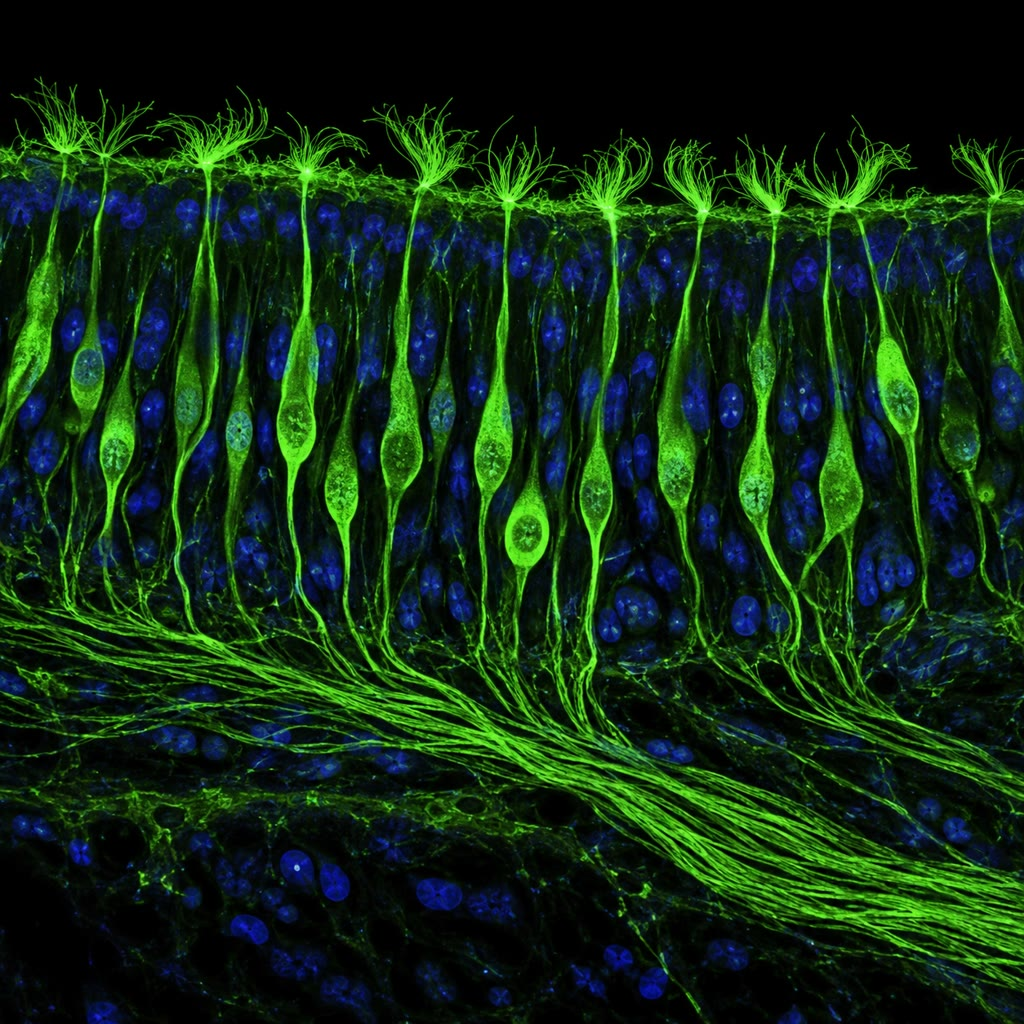
\includegraphics[width=0.40\linewidth]{images/book5/ai/b5-18-olfactory-epithelium.jpg}

{\small El epitelio olfativo: neuronas sensoriales (verde) con
dendritas ciliadas en la superficie, donde se fijan los odorantes, y
axones que se agrupan por debajo camino del bulbo. Cada neurona expresa
un gen de receptor de los cuatrocientos.}
\end{omfigure}

\section{El tacto, la temperatura, el dolor y los sentidos que nos faltan}

\begin{definition}[La somatosensación]\label{def:b3:sensory-systems:somato}
\index{mecanorreceptor}\index{canal Piezo}\index{canal TRP}\index{nociceptor}\index{propiocepción}
La piel alberga varias clases de \emph{mecanorreceptor}, cada una un
axón que termina en su propia cápsula: las células de Merkel para la
presión fina y la textura (de adaptación lenta, campos pequeños), los
corpúsculos de Meissner para el tacto ligero y el deslizamiento (de
adaptación rápida), los corpúsculos de Pacini, profundos en la piel,
para la vibración (de adaptación muy rápida, campos enormes), y las
terminaciones de Ruffini para el estiramiento. El transductor de casi
todos ellos es \emph{Piezo2}, un canal iónico gigante con una hélice de
palas que se abre cuando la membrana se estira; sin él se pierden el
tacto y el sentido de la posición del cuerpo, y el mismo canal, en los
pulmones y en la vejiga, detecta su llenado. La \emph{temperatura} la
detectan canales de la familia TRP ajustados a distintos intervalos
---TRPV1, que abren el calor por encima de \qty{43}{\celsius} y la
capsaicina, y por eso el chile ``pica''; TRPM8, que abren el frío y el
mentol---, y el \emph{dolor}, terminaciones nerviosas libres, los
\emph{nociceptores}, que responden al calor, la presión o los productos
químicos lesivos (protones, ATP, bradicinina) y cuyos umbrales rebaja
la \omterm{def:b3:innate-immunity:inflammation}{inflamación} (\cref{ch:b3:innate-immunity}). La
\emph{propiocepción}, el sentido de dónde están los miembros, procede
de los husos musculares y los órganos tendinosos del
\cref{ch:b3:nervous-systems} y de Piezo2 en las cápsulas articulares.
La densidad de receptores fija la agudeza: dos puntos separados
\qty{2}{mm} se distinguen en la yema de un dedo; en la espalda hace
falta que disten \qty{40}{mm}.
\end{definition}

\begin{method}[Medir un sentido]\label{met:b3:sensory-systems:psychophysics}
\index{psicofísica}\index{umbral}\index{discriminación de dos puntos}
Para caracterizar un canal sensorial: (1) hállese el \emph{umbral
absoluto} presentando muchas veces estímulos de intensidad graduada y
ajustando la fracción detectada ---la intensidad detectada la mitad de
las veces---, como hizo Hecht; (2) hállese el \emph{umbral diferencial}
a varias intensidades y compruébese la \omterm{thm:b3:sensory-systems:weber}{ley de Weber}; (3) cartografíese
la \emph{agudeza espacial} con dos estímulos a separación variable (la
prueba de los dos puntos en la piel, una rejilla en la \omterm{def:b3:sensory-systems:retina}{retina}); (4)
cartografíese la \emph{agudeza temporal} con parpadeos o chasquidos (un
parpadeo se fusiona hacia los \qty{60}{Hz} en la visión diurna); (5) en
un animal, regístrense fibras aferentes aisladas mientras se aplican
los mismos estímulos y háganse coincidir los umbrales neurales con los
conductuales ---la psicofísica y la fisiología deberían concordar, y
allí donde no lo hacen la diferencia es lo que añade el encéfalo.
\end{method}

\begin{remark}[Otros animales, otros sentidos]\label{rem:b3:sensory-systems:others}
Todo sentido tratado aquí tiene una versión que algún animal ha llevado
más lejos, y hay sentidos que nos faltan. Los tiburones y las rayas
perciben los campos de microvoltios del latido de una presa a través de
canales llenos de gelatina; los peces eléctricos leen las distorsiones
de su propio campo para ver en la oscuridad. Las víboras de foseta
forman imágenes de presas calientes con fosetas sensibles al
infrarrojo; los murciélagos y los delfines ecolocalizan, cronometran
los ecos de sus propias llamadas con precisión de unos microsegundos y
gobiernan la frecuencia de la llamada para seguir a una polilla; las
abejas ven el ultravioleta y la polarización de la luz del cielo y se
orientan por ella; las aves migratorias y las tortugas perciben el
campo magnético de la Tierra por un mecanismo todavía discutido. La
nariz de un perro tiene cuarenta veces nuestras neuronas receptoras y
un tercio de su encéfalo para leerlas; un búho oye un ratón bajo la
nieve. Los principios no cambian ---un transductor, una \omterm{def:b3:sensory-systems:principles}{línea marcada},
un código, compresión, un mapa--- y la variedad es lo que la evolución
ha hecho con ellos.
\end{remark}

\section{Ejercicios}

\begin{exercise}[$\star$]\label{exo:b3:sensory-systems:1}
Explíquese cómo sabe el encéfalo si un tren de espigas procede del ojo
o del oído, dado que las espigas son idénticas.
\end{exercise}

\begin{exercise}[$\star$]\label{exo:b3:sensory-systems:2}
¿Por qué la luz hiperpolariza un fotorreceptor y qué es la corriente de
oscuridad?
\end{exercise}

\begin{exercise}[$\star$]\label{exo:b3:sensory-systems:3}
Un susurro tiene \qty{20}{dB}; una conversación, \qty{60}{dB}; un
concierto de rock, \qty{110}{dB}. Calcúlese la intensidad de cada uno
en W/m$^{2}$ y la razón entre el más fuerte y el más suave.
\end{exercise}

\begin{exercise}[$\star$]\label{exo:b3:sensory-systems:4}
Enúnciense las cinco modalidades gustativas y sus tipos de receptor, y
explíquese por qué un resfriado bloquea el ``sabor'' de la comida.
\end{exercise}

\begin{exercise}[$\star\star$]\label{exo:b3:sensory-systems:5}
La fracción de Weber para el peso es $0.02$. Partiendo de un peso de
\qty{100}{g}, ¿cuántos escalones apenas perceptibles hay entre él y
\qty{10}{kg}? Úsese la fórmula de Fechner y compruébese contando
escalones de factor $1.02$.
\end{exercise}

\begin{exercise}[$\star\star$]\label{exo:b3:sensory-systems:6}
Con \cref{thm:b3:sensory-systems:hecht}, calcúlese $P_{\text{ver}}$ para
$a = 2$, $6$ y $12$ fotones absorbidos con un umbral de $n = 6$. ¿Para
qué $a$ se ve el destello la mitad de las veces? Si se absorbe el
\qty{10}{\%} de los fotones que llegan a la córnea, ¿cuántos debe
entregar el destello?
\end{exercise}

\begin{exercise}[$\star\star$]\label{exo:b3:sensory-systems:7}
El oído medio concentra la fuerza desde \qty{55}{mm^2} sobre
\qty{3}{mm^2} con una palanca de $1.3$. ¿Por qué factor se eleva la
presión, y en \omterm{def:b3:sensory-systems:cochlea}{decibelios}? ¿Por qué el oído de una persona con los
huesecillos fusionados (otosclerosis) es más sordo en decenas de
\omterm{def:b3:sensory-systems:cochlea}{decibelios}?
\end{exercise}

\begin{exercise}[$\star\star$]\label{exo:b3:sensory-systems:8}
Explíquese por qué la corriente de transducción de una \omterm{def:b3:sensory-systems:cochlea}{célula ciliada}
aparece en microsegundos mientras que la de un fotorreceptor tarda
decenas de milisegundos, y qué gana cada sentido con su diseño.
\end{exercise}

\begin{exercise}[$\star\star$]\label{exo:b3:sensory-systems:9}
Un ratón tiene \num{1100} tipos de receptor y el ser humano, $400$. Si
un olor activa alrededor del \qty{5}{\%} de los tipos, ¿cuántos
patrones de exactamente ese tamaño tiene disponibles cada uno (úsese
$\binom{R}{k}$ con $k = 0.05R$ y la aproximación de Stirling
$\ln\binom{R}{k} \approx R\,H(k/R)$ con
$H(p) = -p\ln p - (1-p)\ln(1-p)$)?
\end{exercise}

\begin{exercise}[$\star\star\star$]\label{exo:b3:sensory-systems:10}
Un \omterm{def:b3:sensory-systems:retina}{bastón} isomeriza espontáneamente una \omterm{def:b3:sensory-systems:retina}{rodopsina} una vez cada
\qty{40}{s} en la oscuridad. En un grupo de $500$ bastones observado
durante una ventana de \qty{0.1}{s}, ¿cuál es el número medio de
sucesos espontáneos y cuál la probabilidad de que ocurran seis o más
por azar? Explíquese por qué el encéfalo fija el umbral en torno a seis
y no en uno.
\end{exercise}

\begin{exercise}[$\star\star\star$]\label{exo:b3:sensory-systems:11}
El nervio auditivo engancha sus espigas a la fase del sonido hasta
\qty{4}{kHz}, con una fluctuación de unos \qty{20}{\micro s}. El sonido
viaja a \qty{340}{m/s} y los oídos distan \qty{20}{cm}. ¿Cuál es el
mayor retraso interaural, qué resolución angular da una discriminación
de \qty{10}{\micro s} cerca de la línea media y por qué es el código de
lugar, y no el temporal, el que sirve por encima de \qty{4}{kHz}?
\end{exercise}

\begin{exercise}[$\star\star\star$]\label{exo:b3:sensory-systems:12}
La \omterm{def:b3:sensory-systems:principles}{inhibición lateral} hace que un campo gris uniforme junto a otro
oscuro parezca más claro en el borde. Modélese una fila de receptores
excitados cada uno por su propia luz $I_{i}$ e inhibidos por una
fracción $w$ de la de cada vecino,
$r_{i} = I_{i} - w(I_{i-1} + I_{i+1})$, y calcúlese la respuesta a lo
largo de un escalón de $I = 1$ a $I = 2$ con $w = 0.2$. ¿Qué gana y qué
pierde la \omterm{def:b3:sensory-systems:retina}{retina} con esto?
\end{exercise}

\section{Problema: una vela vista de lejos}

\begin{problem}[{Problema de fin de semana --- los fotones de una vela
contados dentro de un ojo lejano, la detección del destello calculada a
partir de la estadística de Poisson y del amplificador del bastón, los
decibelios de un concierto convertidos en movimiento del tímpano y
corriente de célula ciliada, y el código de una nariz enumerado, para
terminar en la distancia a la que se ve la vela, la presión en el
tímpano y los patrones que una nariz puede formar}]
\label{pb:b3:sensory-systems:1}
Datos: una vela emite unos \qty{0.01}{W} de luz visible, a
\qty{550}{nm} (energía del fotón, $3.6\times 10^{-19}$ J). Una pupila
adaptada a la oscuridad mide \qty{7}{mm} de diámetro; la \omterm{def:b3:sensory-systems:retina}{rodopsina}
absorbe el \qty{10}{\%} de los fotones que entran en el ojo; el ojo
integra durante \qty{0.1}{s}; el umbral es de $6$ fotones absorbidos.
Cada fotón absorbido cierra $200$ canales y reduce la corriente de
oscuridad en \qty{1}{pA} durante \qty{0.2}{s}; la corriente de
oscuridad de un \omterm{def:b3:sensory-systems:retina}{bastón} es de \qty{30}{pA}. Sonido: $I_{0} =
\qty{1e-12}{W/m^2}$; el tímpano tiene un área de \qty{55}{mm^2}; un haz
ciliar de \qty{5}{\micro m} de altura se desvía \qty{0.3}{nm} en el
umbral. Olfato: $R = 400$ receptores; la corriente de transducción de
una \omterm{def:b3:sensory-systems:cochlea}{célula ciliada} es de \qty{100}{pA} en saturación.

\medskip
\noindent\textbf{Parte I --- Fotones.}
\begin{enumerate}
  \item ¿Cuántos fotones por segundo emite la vela?
  \item A una distancia $d$ los fotones se reparten sobre una esfera de
        área $4\pi d^{2}$. ¿Cuántos entran en la pupila por segundo a
        \qty{1}{km}? ¿Y a \qty{10}{km}?
  \item ¿Cuántos se absorben en una ventana de integración a cada
        distancia? ¿Se ve la vela (umbral $6$)?
  \item Hállese la distancia a la cual el número medio de absorbidos en
        una ventana vale $6$. Con la estadística de Poisson, ¿qué
        fracción de ventanas supera allí el umbral?
  \item A la distancia de la pregunta 4, ¿cuál es la probabilidad de
        que una ventana dada de \qty{0.1}{s} no contenga fotón alguno?
        ¿Por qué parece parpadear una estrella tenue?
  \item Con luna llena, los mismos bastones absorben $10^{4}$ fotones
        por ventana procedentes del cielo. Explíquese por qué la vela a
        \qty{10}{km} resulta entonces invisible aunque entregue los
        mismos fotones.
\end{enumerate}

\medskip
\noindent\textbf{Parte II --- El amplificador del \omterm{def:b3:sensory-systems:retina}{bastón}.}
\begin{enumerate}[resume]
  \item Un fotón cierra $200$ canales y reduce la corriente en
        \qty{1}{pA}. ¿Qué corriente lleva un canal y cuántos cationes
        por segundo son ($e = \qty{1.6e-19}{C}$)?
  \item ¿Qué fracción de la corriente de oscuridad retira un fotón?
        ¿Cuántos fotones simultáneos apagarían el \omterm{def:b3:sensory-systems:retina}{bastón} por completo
        (saturación)?
  \item La respuesta dura \qty{0.2}{s}. ¿Cuántos cationes impide entrar
        un fotón? ¿Cuál es la ganancia en carga por fotón?
  \item A la luz del día llegan a un \omterm{def:b3:sensory-systems:retina}{bastón} $10^{5}$ fotones por
        segundo. ¿Qué le ocurre, y por qué los \omterm{def:b3:sensory-systems:retina}{conos}, que se adaptan y
        se saturan menos, son los receptores diurnos?
  \item Los \omterm{def:b3:sensory-systems:retina}{conos} necesitan unos $100$ fotones para señalizar.
        Explíquese, en términos del compromiso entre sensibilidad y
        rapidez, por qué los \omterm{def:b3:sensory-systems:retina}{conos} responden en \qty{20}{ms} y los
        bastones en \qty{200}{ms}.
  \item Una \omterm{def:b3:sensory-systems:retina}{rodopsina} se isomeriza espontáneamente una vez cada
        \qty{40}{s}. Sobre los $10^{8}$ bastones de un ojo, ¿cuántos
        fotones falsos por segundo genera la \omterm{def:b3:sensory-systems:retina}{retina} y por qué eso no
        ciega de ruido al ojo adaptado a la oscuridad? (Piénsese en el
        umbral y en el \omterm{def:b3:sensory-systems:principles}{campo receptivo}.)
\end{enumerate}

\medskip
\noindent\textbf{Parte III --- \omterm{def:b3:sensory-systems:cochlea}{Decibelios}.}
\begin{enumerate}[resume]
  \item Un concierto a \qty{110}{dB}: intensidad en W/m$^{2}$ y
        potencia que incide sobre un tímpano.
  \item ¿Cuánta energía acústica recibe el tímpano en un concierto de
        dos horas? Compárese con la energía de una gota de lluvia al
        caer (\qty{1e-4}{J}).
  \item El umbral de audición a \qty{0}{dB}: potencia sobre el tímpano
        y energía por cada \qty{10}{ms} ---compárese con la energía de
        un fotón visible.
  \item El haz ciliar se desvía \qty{0.3}{nm} en el umbral sobre una
        altura de \qty{5}{\micro m}. ¿Qué ángulo es eso, en grados?
        Compárese la desviación con el diámetro de un átomo de
        hidrógeno (\qty{0.1}{nm}).
  \item La exposición prolongada por encima de \qty{85}{dB} daña las
        \omterm{def:b3:sensory-systems:cochlea}{células ciliadas}, y las \omterm{def:b3:sensory-systems:cochlea}{células ciliadas} no se regeneran en los
        mamíferos. Dos horas a \qty{110}{dB} entregan tanta energía
        como cuántas horas a \qty{85}{dB}?
  \item El intervalo de la audición es de \qty{120}{dB}. ¿Cuántos
        escalones apenas perceptibles de sonoridad son, si la fracción
        de Weber para la intensidad vale unos $0.25$ (un \omterm{def:b3:sensory-systems:cochlea}{decibelio})?
\end{enumerate}

\medskip
\noindent\textbf{Parte IV --- El código del olfato.}
\begin{enumerate}[resume]
  \item Con $400$ receptores, cada uno encendido o apagado, ¿cuántos
        patrones hay? Escríbase la respuesta como potencia de diez.
  \item Si un olor activa habitualmente $20$ receptores, ¿cuántos
        patrones distintos de ese tipo hay ($\binom{400}{20}$; úsese
        Stirling o los logaritmos)?
  \item Dos odorantes comparten $15$ de sus $20$ receptores.
        Propóngase una medida de su distancia en el código y
        explíquese por qué huelen parecido.
  \item El ser humano discrimina alrededor de un billón de olores. ¿Qué
        fracción de los patrones de la pregunta 20 es eso, y qué limita
        el número tan por debajo de la capacidad del código?
  \item Un ratón con \num{1100} receptores: ¿cuántos patrones de $20$
        más que un ser humano, como potencia de diez?
  \item Una mutación suprime un gen de receptor. Predígase su efecto
        sobre la capacidad de oler en general y sobre la percepción de
        un odorante que se fija con fuerza a ese receptor (anosmia
        específica).
  \item Resúmase: la distancia a la que se ve la vela (pregunta~4), la
        energía acústica sobre el tímpano en el umbral en \qty{10}{ms}
        (pregunta~15) y el número de patrones de veinte receptores que
        puede formar una nariz humana (pregunta~20).
\end{enumerate}
\end{problem}
